
\newpage
\section{Diseño de la arquitectura de software}

\subsection{Vista de escenarios}

La descripción de la arquitectura se ilustra utilizando un conjunto de casos de uso, o escenarios lo que genera una quinta vista. Los escenarios describen secuencias de interacciones entre objetos, y entre procesos del sistema.

\begin{figure}[H]
\centering
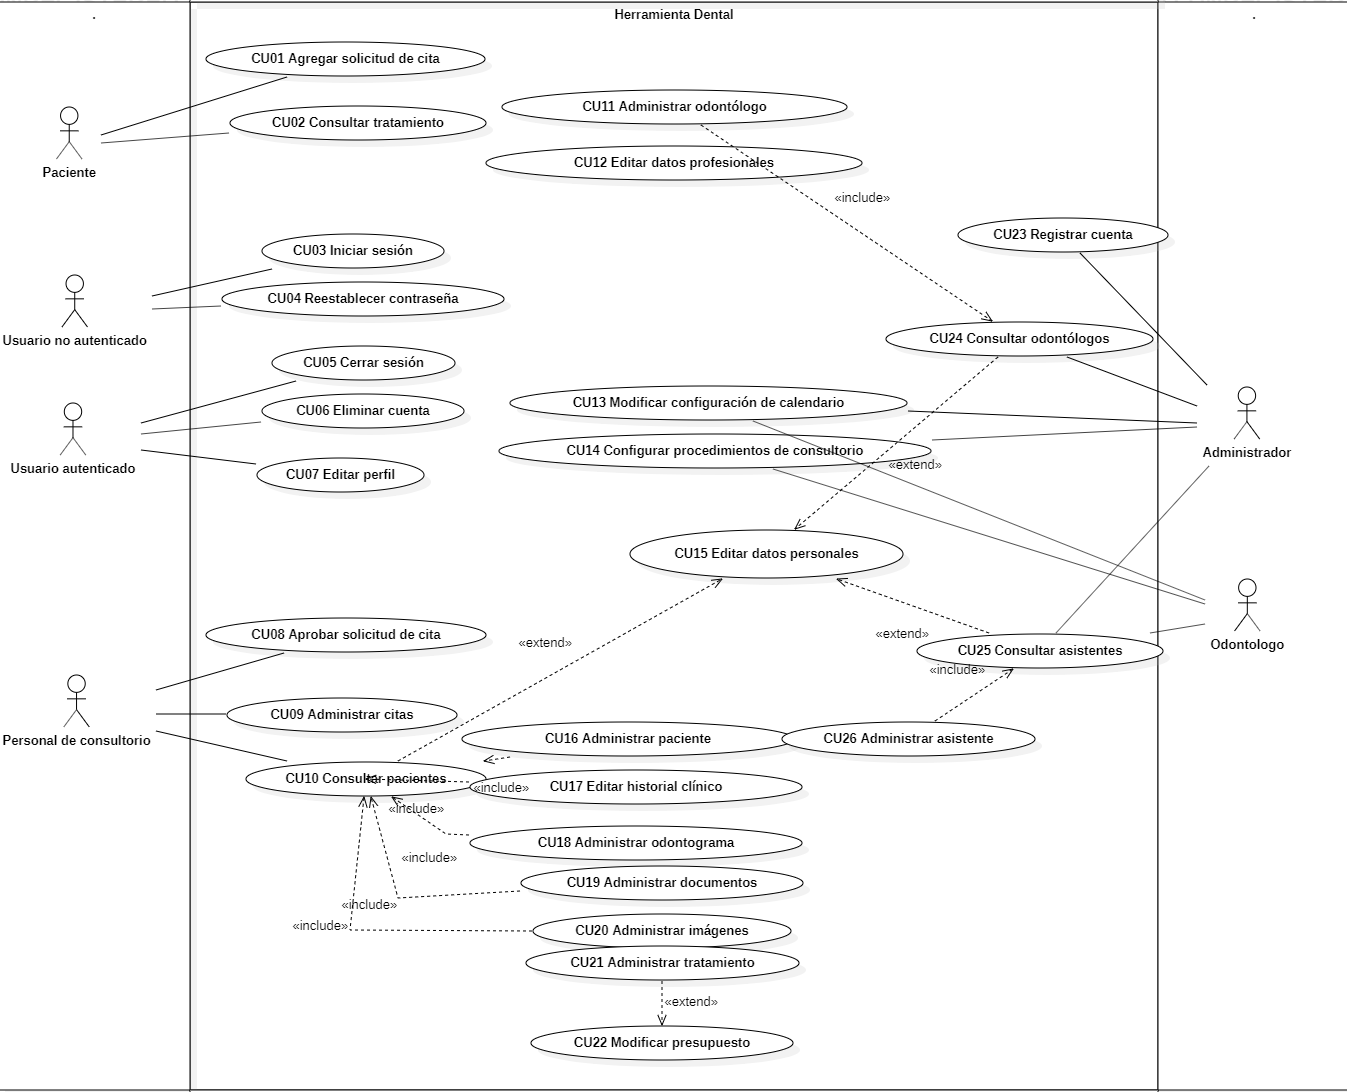
\includegraphics[width=18cm, keepaspectratio]{pictures/herramienta_dental.png}
\caption{Modelo de casos de uso.}
\end{figure}


\newpage
\subsubsection{Actores del sistema}

Se le llama actor a toda entidad externa al sistema que guarda una relación con éste y que le demanda una funcionalidad. Esto incluye a los operadores humanos pero también incluye a todos los sistemas externos, además en ocasiones especiales se incluye de entidades abstractas, como el tiempo.

En el sistema presentado, los actores involucrados son los siguientes.

\begin{figure}[H]
\centering
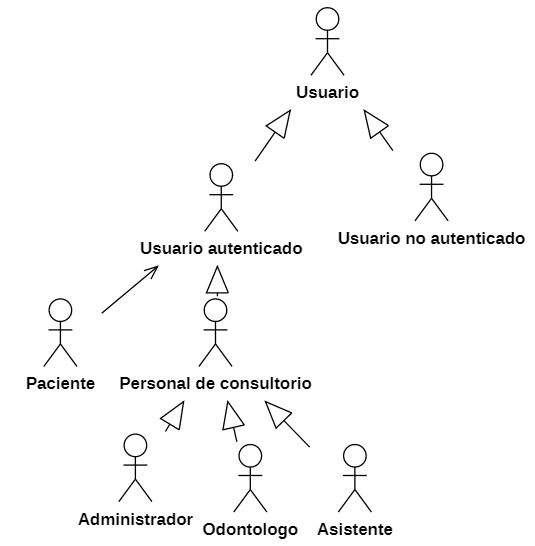
\includegraphics[width=10cm, keepaspectratio]{pictures/actores.JPG}
\caption{Actores involucrados}
\end{figure}

\newpage
\subsubsection{Casos de uso}

%%%%%%%%%%%%%%%%%%%%%%%%%%%%%%%%%%%%%%%%%%%%%


\paragraph{CU01 Agregar solicitud de cita}

\begin{longtable}[H]{|p{0.25\textwidth}|p{12cm}|}
\hline\textbf{ID}         
& \textbf{CU01}            \\ \hline
\textbf{Nombre:}          
& Agregar solicitud de cita       \\ \hline
\textbf{Actor:}          
& Odontólogo, Administrador odontólogo, Paciente   \\ \hline
\textbf{Objetivo:}       
& Permitir al usuario aceptar y agregar las citas pedidas por los pacientes en el sistema.\\ \hline
\textbf{Entradas:}  &             
\begin{itemize}[nosep]
\item Nombre del paciente
\item Apellido paterno del paciente
\item Apellido materno del paciente
\item Fecha de cita
\item Horario de cita
\item Motivo de consulta
\end{itemize}
\\ \hline
\textbf{Salidas:}  &             
\begin{itemize}[nosep]
\item Mensaje de operación exitosa.
\end{itemize}
\\ \hline
\textbf{Precondiciones:}  &             
\begin{itemize}[nosep]
\item El usuario debe estar autenticado en el sistema.
\end{itemize}
\\ \hline
\textbf{Postcondiciones:} &             
\begin{itemize}[nosep]
\item Se registrará la solicitud de cita en el sistema.
\item Se actualizará el listado de las solicitudes de cita para el odontólogo.
\item Se enviará mensaje de envío de solicitud ``Tu solicitud de cita ha sido enviada, recibirás un correo electrónico de confirmación''
\end{itemize}
\\ \hline
\textbf{Errores:}         &             
\begin{minipage}[t]{\linewidth}
\begin{itemize}[nosep]
\item Se muestra el mensaje de error ``Completa el campo obligatorio''
\item Se muestra una pantalla con el mensaje de error ``Error al enviar solicitud de cita.''
\end{itemize}
\vspace{0.2em}
\end{minipage}\\ \hline
\caption{CU01 Agregar solicitud de cita}
\label{table:1}
\end{longtable}

\textbf{Trayectoria principal: Agregar solicitud de cita}
\begin{enumerate}
\item 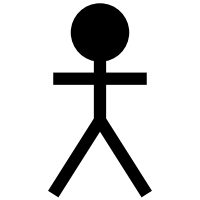
\includegraphics[height=1em]{pictures/actor.png} Solicita registrar una cita.
\item 
\includegraphics[height=1em]{pictures/sistema.png} Muestra una pantalla con el formulario para agendar una cita.
\item 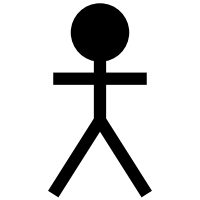
\includegraphics[height=1em]{pictures/actor.png} Para llevar a cabo la solicitud de cita, todos los datos solicitados son completamente obligatorios.
\item 
\includegraphics[height=1em]{pictures/sistema.png} Verifica que se hayan ingresado valores en el campo de texto.
\item 
\includegraphics[height=1em]{pictures/sistema.png} Verifica que los valores ingresados tengan el tipo correcto.
\item 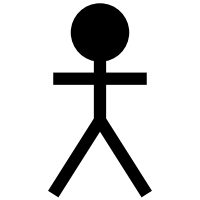
\includegraphics[height=1em]{pictures/actor.png} Da clic en el botón \mybox{Guardar cita}.
\end{enumerate} \bigskip

\textbf{Trayectoria alternativa: Ir a otra opción} 

\vspace{0.3em}

\textbf{Condición:} El usuario no desea proceder con la acción de solicitar una nueva cita.
\begin{enumerate}
\item 
\includegraphics[height=1em]{pictures/sistema.png} El usuario simplemente selecciona otra opción del menú principal.
\end{enumerate} \bigskip

%%%%%%%%%%%%%%%%%%%%%%%%%%%%%%%%%%%%%%%%%%%%%

\paragraph{CU02 Consultar tratamiento}

\begin{longtable}[H]{|p{0.25\textwidth}|p{12cm}|}
\hline\textbf{ID}         
& \textbf{CU02}            \\ \hline
\textbf{Nombre:}          
& Consultar tratamiento       \\ \hline
\textbf{Actor:}          
& Personal de consultorio   \\ \hline
\textbf{Objetivo:}       
& Permitir al usuario visualizar y editar los tratamientos de los pacientes en el sistema.\\ \hline
\textbf{Entradas:}  &  -
\\ \hline
\textbf{Salidas:}  &             
\begin{itemize}[nosep]
\item Listado de tratamientos.
\end{itemize}
\\ \hline
\textbf{Precondiciones:}  &             
\begin{itemize}[nosep]
\item El usuario debe estar autenticado en el sistema.
\item El usuario debe estar en el listado de pacientes del menú "pacientes".
\end{itemize}
\\ \hline
\textbf{Postcondiciones:} & -
\\ \hline
\textbf{Errores:}         &             
\begin{minipage}[t]{\linewidth}

\vspace{0.2em}

\end{minipage}\\ \hline
\caption{CU02 Consultar tratamientos}
\label{table:1}
\end{longtable}

\textbf{Trayectoria principal}
\begin{enumerate}
\item 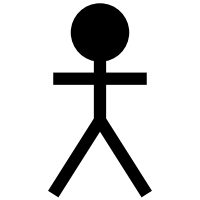
\includegraphics[height=1em]{pictures/actor.png} Selecciona la opción del menú principal "pacientes".
\item 
\includegraphics[height=1em]{pictures/sistema.png} Muestra el listado de pacientes.
\item 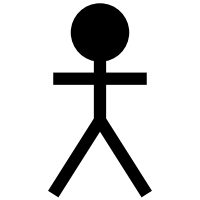
\includegraphics[height=1em]{pictures/actor.png} El usuario selecciona el menú de opciones y le da clic a  \mybox{Tratamientos}.
\item 
\includegraphics[height=1em]{pictures/sistema.png} El sistema le muestra el listado de los tratamientos del paciente en cuestión.
\end{enumerate} \bigskip

\textbf{Trayectoria alternativa: Ir a otra opción} 
\vspace{0.3em}
\textbf{Condición:} El usuario no desea proceder con la acción de ver los tratamientos de un paciente.
\begin{enumerate}
\item 
\includegraphics[height=1em]{pictures/sistema.png} El usuario simplemente selecciona otra opción del menú principal.
\end{enumerate} \bigskip


%%%%%%%%%%%%%%%%%%%%%%%%%%%%%%%%%%%%%%%%%%%%%

\paragraph{CU03 Iniciar sesión}

\begin{longtable}[H]{|p{0.25\textwidth}|p{12cm}|}
\hline\textbf{ID}         
& \textbf{CU03}            \\ \hline
\textbf{Nombre:}          
& Iniciar sesión       \\ \hline
\textbf{Actor:}          
& Usuario no autenticado   \\ \hline
\textbf{Objetivo:}       
& Permitir al usuario no autenticado ingresar e iniciar sesión en el sistema.\\ \hline
\textbf{Entradas:}  &             
\begin{itemize}[nosep]
\item Correo electrónico
\item Contraseña
\end{itemize}
\\ \hline
\textbf{Salidas:}  &             
\begin{itemize}[nosep]
\item Entrada al sistema con el menú principal.
\end{itemize}
\\ \hline
\textbf{Precondiciones:}  &             
\begin{itemize}[nosep]
\item El usuario no autenticado debe estar registrado en el sistema.
\item El usuario no autenticado debe de estar en la página principal.
\end{itemize}
\\ \hline
\textbf{Postcondiciones:} & -
\\ \hline
\textbf{Errores:}         &             
\begin{minipage}[t]{\linewidth}
\begin{itemize}[nosep]
\item Se muestra el mensaje de error ``Completa el campo obligatorio''
\item Se muestra una pantalla con el mensaje de error `` El correo no esta registrado.''
\end{itemize}
\vspace{0.2em}
\end{minipage}\\ \hline
\caption{CU03 Iniciar sesión}
\label{table:1}
\end{longtable}

\textbf{Trayectoria principal: Iniciar sesión}
\begin{enumerate}
\item 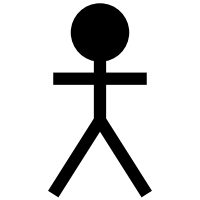
\includegraphics[height=1em]{pictures/actor.png} El usuario registrado no autenticado desea ingresar al sistema y le da clic a "Iniciar sesión".
\item 
\includegraphics[height=1em]{pictures/sistema.png} Muestra una pantalla con el formulario para iniciar sesión.
\item 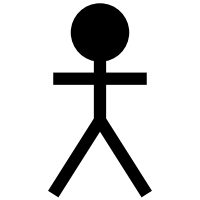
\includegraphics[height=1em]{pictures/actor.png} Para poder iniciar sesión, todos los datos solicitados son completamente obligatorios.
\item 
\includegraphics[height=1em]{pictures/sistema.png} Verifica que se hayan ingresado valores en el campo de texto.
\item 
\includegraphics[height=1em]{pictures/sistema.png} Verifica que los valores ingresados tengan el tipo correcto.
\item 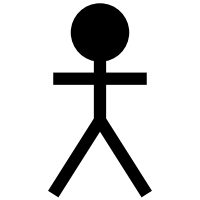
\includegraphics[height=1em]{pictures/actor.png} Da clic en el botón \mybox{Iniciar sesión}.
\end{enumerate} \bigskip

\textbf{Trayectoria alternativa: Ir a "¿Olvidaste tu contraseña?"} 

\vspace{0.3em}

\textbf{Condición:} El usuario no autenticado desea proceder a recuperar su contraseña.
\begin{enumerate}
\item 
\includegraphics[height=1em]{pictures/sistema.png} El sistema lo manda a la pantalla de "¿Olvidaste tu contraseña?."
\end{enumerate} \bigskip

\textbf{Trayectoria alternativa: Ir a "Registrarse"}

\vspace{0.3em}

\textbf{Condición:} El usuario no autenticado desea proceder a registrarse.
\begin{enumerate}
\item 
\includegraphics[height=1em]{pictures/sistema.png} El sistema lo manda a la pantalla de "Registro"
\end{enumerate} \bigskip

\textbf{Trayectoria alternativa: Ir al inicio} 

\vspace{0.3em}

\textbf{Condición:} El usuario no desea proceder con la acción de iniciar sesión.
\begin{enumerate}
\item 
\includegraphics[height=1em]{pictures/sistema.png} El usuario simplemente se va a la página de inicio.
\end{enumerate} \bigskip

%%%%%%%%%%%%%%%%%%%%%%%%%%%%%%%%%%%%%%%%%%%%%

\paragraph{CU04 Restablecer contraseña}

\begin{longtable}[H]{|p{0.25\textwidth}|p{12cm}|}
\hline\textbf{ID}         
& \textbf{CU04}            \\ \hline
\textbf{Nombre:}          
& Restablecer contraseña       \\ \hline
\textbf{Actor:}          
& Usuario no autenticado   \\ \hline
\textbf{Objetivo:}       
& Permitir al usuario no autenticado solicitar la recuperación de contraseña para ingresar en el sistema.\\ \hline
\textbf{Entradas:}  &             
\begin{itemize}[nosep]
\item Correo electrónico.
\end{itemize}
\\ \hline
\textbf{Salidas:}  &             
\begin{itemize}[nosep]
\item Mensaje de operación exitosa "le enviamos un correo a la dirección ingresada.
\end{itemize}
\\ \hline
\textbf{Precondiciones:}  &             
\begin{itemize}[nosep]
\item El usuario debe estar registrado en el sistema.
\end{itemize}
\\ \hline
\textbf{Postcondiciones:} &             
\begin{itemize}[nosep]
\item Se enviará un correo al correo electrónico ingresado en el campo, el cuál contiene un link con un token para restablecer la contraseña.
\item Se enviará mensaje de envío de solicitud ``Correo enviado de forma exitosa.''
\end{itemize}
\\ \hline
\textbf{Errores:}         &             
\begin{minipage}[t]{\linewidth}
\begin{itemize}[nosep]
\item Se muestra el mensaje de error ``Email no registrado ''
\end{itemize}
\vspace{0.2em}
\end{minipage}\\ \hline
\caption{CU04 Restablecer contraseña}
\label{table:1}
\end{longtable}

\textbf{Trayectoria principal: Restablecer contraseña}
\begin{enumerate}
\item 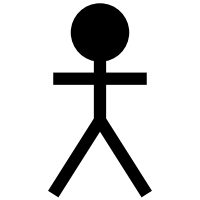
\includegraphics[height=1em]{pictures/actor.png} El usuario no autenticado desea restablecer la contraseña de su cuenta registrada con su correo, se dirige al "¿Olvidaste contraseña?".
\item 
\includegraphics[height=1em]{pictures/sistema.png} Muestra una pantalla con el formulario para restablecer la contraseña.
\item 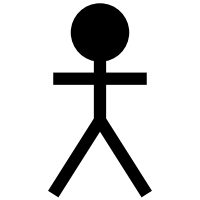
\includegraphics[height=1em]{pictures/actor.png} Para llevar a cabo el restablecimiento de la contraseña, el dato solicitado es completamente obligatorio.
\item 
\includegraphics[height=1em]{pictures/sistema.png} Verifica que se haya ingresado el valor en el campo de texto.
\item 
\includegraphics[height=1em]{pictures/sistema.png} Verifica que el valor ingresado tenga el tipo correcto.
\item 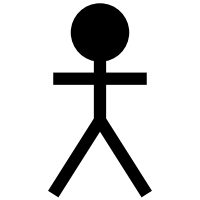
\includegraphics[height=1em]{pictures/actor.png} Da clic en el botón \mybox{Restablecer contraseña}.
\end{enumerate} \bigskip

\textbf{Trayectoria alternativa: Ir a Iniciar Sesión} 

\vspace{0.3em}

\textbf{Condición:} El usuario no desea proceder con el restablecimiento de la contraseña.
\begin{enumerate}
\item 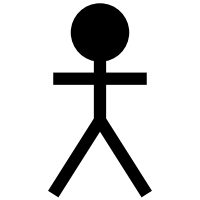
\includegraphics[height=1em]{pictures/actor.png} El usuario simplemente selecciona la opción Iniciar Sesión del menú principal.
\end{enumerate} \bigskip

\textbf{Trayectoria alternativa: Ir a Registrarse} 

\vspace{0.3em}

\textbf{Condición:} El usuario no desea proceder con el restablecimiento de la contraseña.
\begin{enumerate}
\item 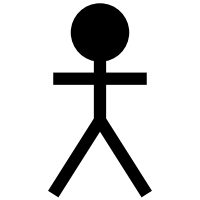
\includegraphics[height=1em]{pictures/actor.png} El usuario simplemente selecciona la opción registrarse del menú principal.
\end{enumerate} \bigskip


%%%%%%%%%%%%%%%%%%%%%%%%%%%%%%%%%%%%%%%%%%%%%

\paragraph{CU05 Cerrar sesión}

\begin{longtable}[H]{|p{0.25\textwidth}|p{12cm}|}
\hline\textbf{ID}         
& \textbf{CU05}            \\ \hline
\textbf{Nombre:}          
& Cerrar sesión       \\ \hline
\textbf{Actor:}          
& Usuario autenticado   \\ \hline
\textbf{Objetivo:}       
& Permitir al usuario autenticado cerrar su sesión en el sistema.\\ \hline
\textbf{Entradas:}  &  -
\\ \hline
\textbf{Salidas:}  &             
\begin{itemize}[nosep]
\item Mensaje de operación exitosa "le enviamos un correo a la dirección ingresada.
\end{itemize}
\\ \hline
\textbf{Precondiciones:}  &             
\begin{itemize}[nosep]
\item El usuario debe estar registrado y autenticado en el sistema.
\end{itemize}
\\ \hline
\textbf{Postcondiciones:} &             
\begin{itemize}[nosep]
\item Se enviará al usuario a la página principal.
\end{itemize}
\\ \hline
\textbf{Errores:}         & - 

\vspace{0.2em}

\caption{CU05 Cerrar sesión}
\label{table:1}
\end{longtable}

\textbf{Trayectoria principal: Cerrar sesión}
\begin{enumerate}
\item 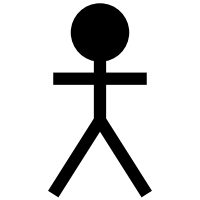
\includegraphics[height=1em]{pictures/actor.png} El usuario autenticado desea cerrar sesión y salirse del sistema.
\item 
\includegraphics[height=1em]{pictures/sistema.png} Muestra una pantalla de inicio.
\end{enumerate} \bigskip


\textbf{Trayectoria alternativa: Ir a otra opción} 

\vspace{0.3em}

\textbf{Condición:} El usuario no desea proceder cerrar su sesión.
\begin{enumerate}
\item 
\includegraphics[height=1em]{pictures/sistema.png} El usuario simplemente selecciona otra opción del menú principal.
\end{enumerate} \bigskip


%%%%%%%%%%%%%%%%%%%%%%%%%%%%%%%%%%%%%%%%%%%%%

\paragraph{CU06 Eliminar cuenta}

\begin{longtable}[H]{|p{0.25\textwidth}|p{12cm}|}
\hline\textbf{ID}         
& \textbf{CU06}            \\ \hline
\textbf{Nombre:}          
& Eliminar cuenta       \\ \hline
\textbf{Actor:}          
& Personal de consultorio   \\ \hline
\textbf{Objetivo:}       
& Permitir al usuario autenticado eliminar su cuenta.\\ \hline
\textbf{Entradas:}  &  -
\\ \hline
\textbf{Salidas:}  &             
\begin{itemize}[nosep]
\item Advertencia para confirmar la eliminación de la cuenta.
\item Se manda al usuario a la página principal y se elimina su cuenta.
\end{itemize}
\\ \hline
\textbf{Precondiciones:}  &             
\begin{itemize}[nosep]
\item El usuario debe estar registrado en el sistema.
\end{itemize}
\\ \hline
\textbf{Postcondiciones:} &             
\begin{itemize}[nosep]
\item Se envía al usuario a la página principal del sistema
\end{itemize}
\\ \hline
\textbf{Errores:}         &             
\begin{minipage}[t]{\linewidth} -

\vspace{0.2em}

\end{minipage}\\ \hline
\caption{CU06 Eliminar cuenta}
\label{table:1}
\end{longtable}

\textbf{Trayectoria principal: Eliminar cuenta de administrador odontólogo}
\begin{enumerate}
\item 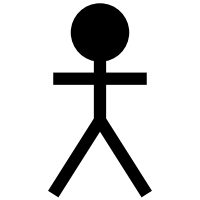
\includegraphics[height=1em]{pictures/actor.png} El administrador odontólogo desea eliminar su cuenta y se va a al menú con un icono de una persona y se dirige al menú contextual de datos personales.
\item 
\includegraphics[height=1em]{pictures/sistema.png} Muestra una pantalla con los campos de los datos personales y el botón de \mybox{Eliminar cuenta} .
\item 
\includegraphics[height=1em]{pictures/sistema.png} Para llevar a cabo la eliminación de la cuenta, se le muestra una confirmación al administrador odontólogo para eliminar la cuenta.
\item 
\includegraphics[height=1em]{pictures/sistema.png} El sistema elimina de la lista de administradores odontólogos al usuario seleccionado.
\end{enumerate} \bigskip

\textbf{Trayectoria principal: Eliminar cuenta de paciente}
\begin{enumerate}
\item 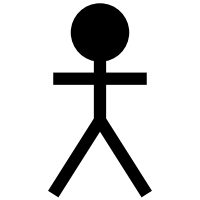
\includegraphics[height=1em]{pictures/actor.png} El personal de consultorio desea eliminar una cuenta de algún paciente y se va a al menú de pacientes.
\item 
\includegraphics[height=1em]{pictures/sistema.png} Muestra una pantalla con la lista de los pacientes.
\item 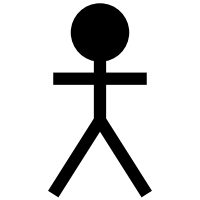
\includegraphics[height=1em]{pictures/actor.png} Para llevar a cabo la eliminación de la cuenta, se da clic en las opciones y se le da clic en \mybox{Eliminar}.
\item 
\includegraphics[height=1em]{pictures/sistema.png} El sistema elimina de la lista de pacientes al usuario seleccionado.
\end{enumerate} \bigskip

\textbf{Trayectoria principal: Eliminar cuenta de odontólogo}
\begin{enumerate}
\item 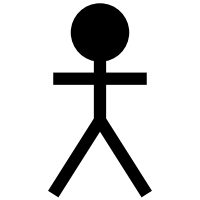
\includegraphics[height=1em]{pictures/actor.png} El personal de consultorio desea eliminar una cuenta de algún odontólogo y se va a al menú de odontólogo.
\item 
\includegraphics[height=1em]{pictures/sistema.png} Muestra una pantalla con la lista de los odontólogos.
\item 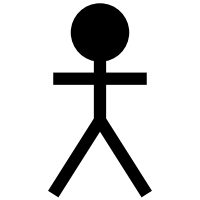
\includegraphics[height=1em]{pictures/actor.png} Para llevar a cabo la eliminación de la cuenta, se da clic en las opciones y se le da clic en \mybox{Eliminar}.
\item 
\includegraphics[height=1em]{pictures/sistema.png} El sistema elimina de la lista de odontólogos al usuario seleccionado.
\end{enumerate} \bigskip


\textbf{Trayectoria principal: Eliminar cuenta de asistente}
\begin{enumerate}
\item 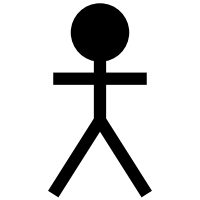
\includegraphics[height=1em]{pictures/actor.png} El personal de consultorio desea eliminar una cuenta de algún asistente y se va a al menú de asistentes.
\item 
\includegraphics[height=1em]{pictures/sistema.png} Muestra una pantalla con la lista de los asistentes.
\item 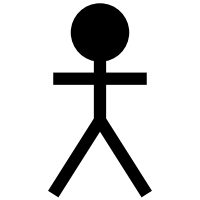
\includegraphics[height=1em]{pictures/actor.png} Para llevar a cabo la eliminación de la cuenta, se da clic en las opciones y se le da clic en \mybox{Eliminar}.
\item 
\includegraphics[height=1em]{pictures/sistema.png} El sistema elimina de la lista de asistentes al usuario seleccionado.
\end{enumerate} \bigskip



\textbf{Trayectoria alternativa: Ir a otra opción} 

\vspace{0.3em}

\textbf{Condición:} El usuario no desea proceder con la eliminación de la cuenta.
\begin{enumerate}
\item \includegraphics[height=1em]{pictures/actor.png} El usuario simplemente selecciona otra opción.
\end{enumerate} \bigskip


%%%%%%%%%%%%%%%%%%%%%%%%%%%%%%%%%%%%%%%%%%%%%

\paragraph{CU07 Editar perfil}

\begin{longtable}[H]{|p{0.25\textwidth}|p{12cm}|}
\hline\textbf{ID}         
& \textbf{CU07}            \\ \hline
\textbf{Nombre:}          
& Editar perfil       \\ \hline
\textbf{Actor:}          
& Administrador Odontólogo   \\ \hline
\textbf{Objetivo:}       
& Permitir al usuario Editar sus datos.\\ \hline
\textbf{Entradas:}  &             
\begin{itemize}[nosep]
\item Nombre
\item Primer apellido
\item Segundo apellido
\item Correo electrónico
\item RFC
\item Teléfono fijo
\item Teléfono móvil
\item Fecha de nacimiento
\item Género
\end{itemize}
\\ \hline
\textbf{Salidas:}  &             
\begin{itemize}[nosep]
\item Pantalla principal.
\end{itemize}
\\ \hline
\textbf{Precondiciones:}  &             
\begin{itemize}[nosep]
\item El usuario debe estar registrado y autenticado en el sistema.
\end{itemize}
\\ \hline
\textbf{Postcondiciones:} &
\begin{itemize}[nosep]
\item El usuario es mandado a la página de inicio.
\end{itemize}
\\ \hline
\textbf{Errores:}         &             
\begin{minipage}[t]{\linewidth}
\begin{itemize}[nosep]
\item Se muestra el mensaje de error ``Completa el campo obligatorio''
\end{itemize}
\vspace{0.2em}
\end{minipage}\\ \hline
\caption{CU07 Editar perfil}
\label{table:1}
\end{longtable}

\textbf{Trayectoria principal: Editar perfil}
\begin{enumerate}
\item \includegraphics[height=1em]{pictures/actor.png} El usuario registrado autenticado desea editar sus datos personales y le da clic a "Perfil".
\item \includegraphics[height=1em]{pictures/sistema.png} Muestra una pantalla con el formulario para editar datos personales del perfil.
\item \includegraphics[height=1em]{pictures/actor.png} Para poder editar datos personales, los datos se pueden ir editando.
\item \includegraphics[height=1em]{pictures/sistema.png} Verifica que se hayan ingresado valores en el campo de texto.
\item \includegraphics[height=1em]{pictures/sistema.png} El sistema los guarda y manda a la pantalla principal.
\end{enumerate} \bigskip


\textbf{Trayectoria alternativa: Ir al inicio} 

\vspace{0.3em}

\textbf{Condición:} El usuario no desea proceder con la acción de editar perfil.
\begin{enumerate}
\item \includegraphics[height=1em]{pictures/sistema.png} El usuario simplemente se va a la página de inicio.
\end{enumerate} \bigskip

%%%%%%%%%%%%%%%%%%%%%%%%%%%%%%%%%%%%%%%%%%%%%
\paragraph{CU08 Aprobar solicitud de cita}

\begin{longtable}[H]{|p{0.25\textwidth}|p{12cm}|}
\hline\textbf{ID}         
& \textbf{CU08}            \\ \hline
\textbf{Nombre:}          
& Agregar solicitud de cita       \\ \hline
\textbf{Actor:}          
& Odontólogo, Administrador odontólogo   \\ \hline
\textbf{Objetivo:}       
& Permitir al usuario aprobar y agregar las citas pedidas por los pacientes en el sistema.\\ \hline
\textbf{Entradas:}  &             
\begin{itemize}[nosep]
\item Nombre del paciente
\item Apellido paterno del paciente
\item Apellido materno del paciente
\item Fecha de cita
\item Horario de cita
\item Motivo de consulta
\end{itemize}
\\ \hline
\textbf{Salidas:}  &             
\begin{itemize}[nosep]
\item Cita agendada.
\end{itemize}
\\ \hline
\textbf{Precondiciones:}  &             
\begin{itemize}[nosep]
\item El usuario que solicita una cita y el usuario que la acepta deben estar autenticados en el sistema.
\end{itemize}
\\ \hline
\textbf{Postcondiciones:} &             
\begin{itemize}[nosep]
\item Se enviará la solicitud de cita en la agenda de el sistema.
\item Se actualizará el listado de las solicitudes de cita para el odontólogo.
\item Se enviará mensaje de aprobación o rechazo de la cita.
\end{itemize}
\\ \hline
\textbf{Errores:}         &             
\begin{minipage}[t]{\linewidth}
\begin{itemize}[nosep]
\item Se muestra un mensaje de error.
\end{itemize}
\vspace{0.2em}
\end{minipage}\\ \hline
\caption{CU08 Aprobar solicitud de cita}
\label{table:1}
\end{longtable}

\textbf{Trayectoria principal: Aprobar solicitud de cita}
\begin{enumerate}
\item \includegraphics[height=1em]{pictures/actor.png} El odontólogo o administrador odontólogo acepta la cita dando clic al botón  \mybox{Aceptar}.
\item \includegraphics[height=1em]{pictures/sistema.png} Muestra una pantalla con la aprobación de una cita y se agrega a la agenda del odontólogo correspondiente.
\item \includegraphics[height=1em]{pictures/sistema.png} El sistema envía un correo de aprobación de cita para el correo registrado del paciente que solicita la cita.
\end{enumerate} \bigskip

\textbf{Trayectoria principal: Rechazar solicitud de cita}
\begin{enumerate}
\item \includegraphics[height=1em]{pictures/actor.png} El odontólogo o administrador odontólogo rechaza la cita dando clic al botón  \mybox{Eliminar}.
\item \includegraphics[height=1em]{pictures/sistema.png} Muestra una pantalla con la cita eliminada y se borra del sistema.

\end{enumerate} \bigskip

\textbf{Trayectoria alternativa: Ir a otra opción} 

\vspace{0.3em}

\textbf{Condición:} El usuario no desea proceder y se dirige a otra opción.
\begin{enumerate}
\item \includegraphics[height=1em]{pictures/sistema.png} El usuario simplemente selecciona otra opción del menú principal.
\end{enumerate} \bigskip

%%%%%%%%%%%%%%%%%%%%%%%%%%%%%%%%%%%%%%%%%%%%%

%%%%%%%%%%%%%%%%%%%%%%%%%%%%%%%%%%%%%%%%%%%%%

\paragraph{CU09 Administrar citas}

\begin{longtable}[H]{|p{0.25\textwidth}|p{12cm}|}
\hline\textbf{ID}         
& \textbf{CU09}            \\ \hline
\textbf{Nombre:}          
& Administrar citas      \\ \hline
\textbf{Actor:}          
& Administrador de consultorio (Administrador odontólogo), Odontólogo, asistente   \\ \hline
\textbf{Objetivo:}       
& Permitir al personal de consultorio, registrar, consultar, modificar, o eliminar las citas en el sistema.\\ \hline
\textbf{Entradas:}  &             
\begin{itemize}[nosep]
\item Paciente
\item Motivo de consulta
\item Fecha
\item Hora
\item Duración
\item Observaciones
\end{itemize}
\\ \hline
\textbf{Salidas:}  &             
\begin{itemize}[nosep]
\item Mensaje de operación exitosa.
\end{itemize}
\\ \hline
\textbf{Precondiciones:}  &             
\begin{itemize}[nosep]
\item El usuario debe estar autenticado en el sistema.
\end{itemize}
\\ \hline
\textbf{Postcondiciones:} &             
\begin{itemize}[nosep]
\item Se registrará en el sistema un nueva cita.
\item Se actualizará el listado de citas.
\end{itemize}
\\ \hline
\textbf{Errores:}         &             
\begin{minipage}[t]{\linewidth}
\begin{itemize}[nosep]
\item Se muestra el mensaje de error ``Completa el campo obligatorio''
\item Se muestra una pantalla con el mensaje de error ``Tipo de dato incorrecto.''
\end{itemize}
\vspace{0.2em}
\end{minipage}\\ \hline
\caption{CU09 Administrar citas}
\label{table:1}
\end{longtable}

\textbf{Trayectoria principal: Registrar cita}  
\begin{enumerate}
\item \includegraphics[height=1em]{pictures/actor.png} Solicita registrar una nueva cita.
\item \includegraphics[height=1em]{pictures/sistema.png} Muestra una pantalla con el formulario de registro de datos de la cita.
\item \includegraphics[height=1em]{pictures/actor.png} Para llevar a cabo el registro de una nueva cita, los datos solicitados, el paciente seleccionado, el motivo de consulta, la fecha, la hora y la duración son completamente obligatorios.
\item \includegraphics[height=1em]{pictures/sistema.png} Verifica que se hayan ingresado valores en el campo de texto.
\item \includegraphics[height=1em]{pictures/sistema.png} Verifica que los valores ingresados tengan el tipo correcto.
\item \includegraphics[height=1em]{pictures/actor.png} Da clic en el botón \mybox{Guardar Cita}.
\end{enumerate} \bigskip

\textbf{Trayectoria principal: Modificar/Consultar cita}        
\begin{enumerate}
\item \includegraphics[height=1em]{pictures/actor.png} Se seleccionan las citas dentro de un calendario con una agenda.
\item \includegraphics[height=1em]{pictures/sistema.png} Se elige la opción modificar cita.
\item \includegraphics[height=1em]{pictures/actor.png} Se realiza modificación de los datos de la cita.
\item \includegraphics[height=1em]{pictures/sistema.png} Verifica que se hayan ingresado valores en el campo de texto.
\item \includegraphics[height=1em]{pictures/sistema.png} Verifica que los valores ingresados tengan el tipo correcto.
\item \includegraphics[height=1em]{pictures/actor.png} Da clic en el botón \mybox{Guardar Cita}.
\end{enumerate} \bigskip

\textbf{Trayectoria principal: Eliminar cita}        
\begin{enumerate}
\item \includegraphics[height=1em]{pictures/actor.png} Se seleccionan la cita a eliminar.
\item \includegraphics[height=1em]{pictures/sistema.png} Se elige la opción eliminar.
\item \includegraphics[height=1em]{pictures/sistema.png} Se muestra una pantalla con el mensaje ``Cita eliminada.''
\end{enumerate} \bigskip


\textbf{Trayectoria alternativa: Cancelar registro de cita} \bigskip
\vspace{0.3em}
\textbf{Condición:} El usuario no desea proceder con la acción de agregar una nueva cita.
\begin{enumerate}
\item \includegraphics[height=1em]{pictures/sistema.png} El usuario simplemente selecciona otra opción del menú principal.
\end{enumerate} \bigskip
%%%%%%%%%%%%%%%%%%%%%%%%%%%%%%%%%%%%%%%%%%%%%


\paragraph{CU10 Consultar pacientes}

\begin{longtable}[H]{|p{0.25\textwidth}|p{12cm}|}
\hline\textbf{ID}         
& \textbf{CU10}            \\ \hline
\textbf{Nombre:}          
& Consultar pacientes      \\ \hline
\textbf{Actor:}          
& Personal de consultorio   \\ \hline
\textbf{Objetivo:}       
& Permitir al usuario consultar el listado de pacientes asociados a  un consultorio.\\ \hline
\textbf{Entradas:}  &   -
\\ \hline
\textbf{Salidas:}  &             
\begin{itemize}[nosep]
\item Listado de pacientes.
\end{itemize}
\\ \hline
\textbf{Precondiciones:}  &             
\begin{itemize}[nosep]
\item El usuario debe estar autenticado en el sistema.
\end{itemize}
\\ \hline
\textbf{Postcondiciones:} &  -
\\ \hline 
\textbf{Errores:} &  -
\\ \hline
\caption{CU10 Consultar pacientes}
\label{table:1}
\end{longtable}

\textbf{Trayectoria principal}
\begin{enumerate}
\item \includegraphics[height=1em]{pictures/actor.png} Selecciona la opción del menú principal ``pacientes".
\item \includegraphics[height=1em]{pictures/sistema.png} Muestra una pantalla con el listado completo pacientes del consultorio.
\end{enumerate} \bigskip

%%%%%%%%%%%%%%%%%%%%%%%%%%%%%%%%%%%%%%%%%%%%%

\paragraph{CU11 Administrar odontólogo}

\begin{longtable}[H]{|p{0.25\textwidth}|p{12cm}|}
\hline\textbf{ID}         
& \textbf{CU11}            \\ \hline
\textbf{Nombre:}          
& Administrar odontólogo      \\ \hline
\textbf{Actor:}          
& Administrador de consultorio (Administrador odontólogo)   \\ \hline
\textbf{Objetivo:}       
& Permitir al administrador registrar, consultar, modificar, o eliminar la información de los odontólogos en el sistema.\\ \hline
\textbf{Entradas:}  &             
\begin{itemize}[nosep]
\item Datos personales de odontólogo
\end{itemize}
\\ \hline
\textbf{Salidas:}  &             
\begin{itemize}[nosep]
\item Mensaje de operación exitosa.
\end{itemize}
\\ \hline
\textbf{Precondiciones:}  &             
\begin{itemize}[nosep]
\item El usuario debe estar autenticado en el sistema.
\end{itemize}
\\ \hline
\textbf{Postcondiciones:} &             
\begin{itemize}[nosep]
\item Se registrará en el sistema un nuevo paciente.
\item Se actualizará el listado de pacientes.
\end{itemize}
\\ \hline
\textbf{Errores:}         &             
\begin{minipage}[t]{\linewidth}
\begin{itemize}[nosep]
\item Se muestra el mensaje de error ``Completa el campo obligatorio''
\item Se muestra una pantalla con el mensaje de error ``Tipo de dato incorrecto.''
\end{itemize}
\vspace{0.2em}
\end{minipage}\\ \hline
\caption{CU11 Administrar odontólogo}
\label{table:1}
\end{longtable}

\textbf{Trayectoria principal: Registrar odontólogo}  
\begin{enumerate}
\item \includegraphics[height=1em]{pictures/actor.png} Solicita registrar un nuevo odontólogo.
\item \includegraphics[height=1em]{pictures/sistema.png} Muestra una pantalla con el formulario de registro de datos personales del odontólogo.
\item \includegraphics[height=1em]{pictures/actor.png} Para llevar a cabo el registro de un nuevo odontólogo, los datos solicitados, con solo el nombre,apellidos y correo son completamente obligatorios.
\item \includegraphics[height=1em]{pictures/sistema.png} Verifica que se hayan ingresado valores en el campo de texto.
\item \includegraphics[height=1em]{pictures/sistema.png} Verifica que los valores ingresados tengan el tipo correcto.
\item \includegraphics[height=1em]{pictures/actor.png} Da clic en el botón \mybox{Guardar}.
\end{enumerate} \bigskip

\textbf{Trayectoria principal: Modificar/Consultar odontólogo}        
\begin{enumerate}
\item \includegraphics[height=1em]{pictures/actor.png} Se seleccionan las acciones de un odontólogo.
\item \includegraphics[height=1em]{pictures/sistema.png} Se elige la opción modificar datos personales.
\item \includegraphics[height=1em]{pictures/actor.png} Se realiza modificación de los datos y/o profesionales.
\item \includegraphics[height=1em]{pictures/sistema.png} Verifica que se hayan ingresado valores en el campo de texto.
\item \includegraphics[height=1em]{pictures/sistema.png} Verifica que los valores ingresados tengan el tipo correcto.
\item \includegraphics[height=1em]{pictures/actor.png} Da clic en el botón \mybox{Guardar}.
\end{enumerate} \bigskip

\textbf{Trayectoria principal: Eliminar odontólogo}        
\begin{enumerate}
\item \includegraphics[height=1em]{pictures/actor.png} Se seleccionan las acciones de un odontólogo.
\item \includegraphics[height=1em]{pictures/sistema.png} Se elige la opción eliminar.
\item \includegraphics[height=1em]{pictures/sistema.png} Se muestra una pantalla con el mensaje ``Odontólogo eliminado.''
\end{enumerate} \bigskip


\textbf{Trayectoria alternativa: Cancelar registro de odontólogo} \bigskip
\vspace{0.3em}
\textbf{Condición:} El usuario no desea proceder con la acción de agregar paciente nuevo.
\begin{enumerate}
\item \includegraphics[height=1em]{pictures/sistema.png} El usuario simplemente selecciona otra opción del menú principal.
\end{enumerate} \bigskip





%%%%%%%%%%%%%%%%%%%%%%%%%%%%%%%%%%%%%%%%%%%%%

\paragraph{CU12 Editar datos profesionales}

\begin{longtable}[H]{|p{0.25\textwidth}|p{12cm}|}
\hline\textbf{ID}         
& \textbf{CU12}            \\ \hline
\textbf{Nombre:}          
& Editar datos profesionales      \\ \hline
\textbf{Actor:}          
& Personal de consultorio   \\ \hline
\textbf{Objetivo:}       
& Permitir al usuario consultar y modificar datos profesionales de odontólogos en el sistema.\\ \hline
\textbf{Entradas:}  &             
\begin{itemize}[nosep]
\item RFC
\item Cédula profesional
\item Especialidad
\end{itemize}
\\ \hline
\textbf{Salidas:}  &    -
\\ \hline
\textbf{Precondiciones:}  &             
\begin{itemize}[nosep]
\item El usuario debe estar autenticado en el sistema.
\end{itemize}
\\ \hline
\textbf{Postcondiciones:} &             
\begin{itemize}[nosep]
\item Se editará algunos datos profesionales de un odontólogo en el sistema .
\end{itemize}
\\ \hline
\textbf{Errores:}         &             
\begin{minipage}[t]{\linewidth}
\begin{itemize}[nosep]
\item Se muestra el mensaje de error ``Completa el campo obligatorio''
\item Se muestra una pantalla con el mensaje de error ``Tipo de dato incorrecto.''
\end{itemize}
\vspace{0.2em}
\end{minipage}\\ \hline
\caption{CU12 Editar datos profesionales}
\label{table:1}
\end{longtable}


\textbf{Trayectoria principal: Modificar/Consultar datos profesionales de odontólogo}    
\begin{enumerate}
\item \includegraphics[height=1em]{pictures/actor.png} Se selecciona de las acciones un odontólogo cualquiera la opción "Datos personales".
\item \includegraphics[height=1em]{pictures/sistema.png} Muestra una pantalla con los datos en los cuales se incluyen tanto datos de contacto (datos personales) como datos profesionales.
\item \includegraphics[height=1em]{pictures/actor.png} Se realiza modificación de los datos.
\item \includegraphics[height=1em]{pictures/sistema.png} Verifica que se hayan ingresado valores en el campo de texto.
\item \includegraphics[height=1em]{pictures/sistema.png} Verifica que los valores ingresados tengan el tipo correcto.
\item \includegraphics[height=1em]{pictures/actor.png} Da clic en el botón \mybox{Guardar}.
\end{enumerate} \bigskip



%%%%%%%%%%%%%%%%%%%%%%%%%%%%%%%%%%%%%%%%%%%%%

\paragraph{CU13 Modificar configuración de calendario}
\begin{longtable}[H]{|p{0.25\textwidth}|p{12cm}|}
\hline\textbf{ID}         
& \textbf{CU13}            \\ \hline
\textbf{Nombre:}          
& CU13 Modificar configuración de calendario      \\ \hline
\textbf{Actor:}          
& Personal de consultorio   \\ \hline
\textbf{Objetivo:}       
& Permitir al usuario agregar, eliminar o cambiar los horarios activos de trabajo de un odontólogo asociado al usuario. Por ejemplo en el caso de administrador odontólogo y odontólogo, es el propio, pero en caso de asistente es el horario de su odontólogo al cual está asociado.\\ \hline
\textbf{Entradas:}  &             
\begin{itemize}[nosep]
\item Horario de trabajo
\end{itemize}
\\ \hline
\textbf{Salidas:}  &    -
\\ \hline
\textbf{Precondiciones:}  &             
\begin{itemize}[nosep]
\item El usuario debe estar autenticado en el sistema.
\end{itemize}
\\ \hline
\textbf{Postcondiciones:} &             
\begin{itemize}[nosep]
\item Se modificaran los datos del horario de trabajo de un odontólogo.
\end{itemize}
\\ \hline
\textbf{Errores:}         &             
\begin{minipage}[t]{\linewidth}
\begin{itemize}[nosep]
\item Se muestra el mensaje de error ``Completa el campo obligatorio''
\end{itemize}
\vspace{0.2em}
\end{minipage}\\ \hline
\caption{CU13 Modificar configuración de calendario}
\label{table:1}
\end{longtable}

\textbf{Trayectoria principal}
\begin{enumerate}
\item \includegraphics[height=1em]{pictures/actor.png} Se selecciona la opción de agenda en el menú de opciones.
\item \includegraphics[height=1em]{pictures/sistema.png} Muestra una vista de calendario con las opciones "Agregar cita" y "Configurar calendario"
\item \includegraphics[height=1em]{pictures/actor.png} Selecciona la opción "Configurar calendario".
\item \includegraphics[height=1em]{pictures/actor.png} Agrega o modifica inputs del horario y día activo, pudiendo agregar intervalos de hora asociados a un día, el cuál puede marcar como hábil o inhábil.
\item \includegraphics[height=1em]{pictures/sistema.png} Verifica que se hayan ingresado valores en el campo de texto.
\item \includegraphics[height=1em]{pictures/actor.png} Da clic en el botón \mybox{Guardar}.
\end{enumerate} \bigskip


%%%%%%%%%%%%%%%%%%%%%%%%%%%%%%%%%%%%%%%%%%%%%

\paragraph{CU14 Configurar procedimientos de consultorio}
\begin{longtable}[H]{|p{0.25\textwidth}|p{12cm}|}
\hline\textbf{ID}         
& \textbf{CU14}            \\ \hline
\textbf{Nombre:}          
& Configurar procedimientos de consultorio      \\ \hline
\textbf{Actor:}          
& Personal de consultorio   \\ \hline
\textbf{Objetivo:}       
& Permitir al usuario agregar, eliminar o cambiar datos del catálogo de procedimientos y conceptos del consultorio.\\ \hline
\textbf{Entradas:}  &             
\begin{itemize}[nosep]
\item Concepto
\item Precio
\end{itemize}
\\ \hline
\textbf{Salidas:}  &    -
\\ \hline
\textbf{Precondiciones:}  &             
\begin{itemize}[nosep]
\item El usuario debe estar autenticado en el sistema.
\end{itemize}
\\ \hline
\textbf{Postcondiciones:} &             
\begin{itemize}[nosep]
\item Se agregarán, eliminarán o modificarán elementos del catálogo de procedimientos y conceptos.
\end{itemize}
\\ \hline
\textbf{Errores:}         &             
\begin{minipage}[t]{\linewidth}
\begin{itemize}[nosep]
\item Se muestra el mensaje de error ``Completa el campo obligatorio''
\item Se muestra una pantalla con el mensaje de error ``Tipo de dato incorrecto.''
\end{itemize}
\vspace{0.2em}
\end{minipage}\\ \hline
\caption{CU14 Configurar procedimientos de consultorio}
\label{table:1}
\end{longtable}

\textbf{Trayectoria principal}
\begin{enumerate}
\item \includegraphics[height=1em]{pictures/actor.png} Se selecciona de las acciones un paciente cualquiera la opción "tratamientos".
\item \includegraphics[height=1em]{pictures/sistema.png} Muestra una pantalla con la lista de tratamientos de un paciente.
\item \includegraphics[height=1em]{pictures/actor.png} Selecciona la opción "Agregar tratamiento".
\item \includegraphics[height=1em]{pictures/actor.png} Selecciona la opción "Configurar procedimientos".
\item \includegraphics[height=1em]{pictures/actor.png} Agrega o modifica inputs de conceptos con su respectivo precio para el catálogo de procedimientos.
\item \includegraphics[height=1em]{pictures/sistema.png} Verifica que se hayan ingresado valores en el campo de texto.
\item \includegraphics[height=1em]{pictures/sistema.png} Verifica que los valores ingresados tengan el tipo correcto.
\item \includegraphics[height=1em]{pictures/actor.png} Da clic en el botón \mybox{Guardar}.
\end{enumerate} \bigskip

%%%%%%%%%%%%%%%%%%%%%%%%%%%%%%%%%%%%%%%%%%%%%

\paragraph{CU15 Editar datos personales}

\begin{longtable}[H]{|p{0.25\textwidth}|p{12cm}|}
\hline\textbf{ID}         
& \textbf{CU15}            \\ \hline
\textbf{Nombre:}          
& Editar datos personales      \\ \hline
\textbf{Actor:}          
& Personal de consultorio   \\ \hline
\textbf{Objetivo:}       
& Permitir al usuario consultar y modificar datos personales de otros usuarios en el sistema.\\ \hline
\textbf{Entradas:}  &             
\begin{itemize}[nosep]
\item RFC
\item Teléfono fijo
\item Teléfono movil
\item Correo electrónico
\item Fecha de nacimiento
\item Género
\end{itemize}
\\ \hline
\textbf{Salidas:}  &    -
\\ \hline
\textbf{Precondiciones:}  &             
\begin{itemize}[nosep]
\item El usuario debe estar autenticado en el sistema.
\end{itemize}
\\ \hline
\textbf{Postcondiciones:} &             
\begin{itemize}[nosep]
\item Se editará algunos datos personales de un usuario en el sistema .
\end{itemize}
\\ \hline
\textbf{Errores:}         &             
\begin{minipage}[t]{\linewidth}
\begin{itemize}[nosep]
\item Se muestra el mensaje de error ``Completa el campo obligatorio''
\item Se muestra una pantalla con el mensaje de error ``Tipo de dato incorrecto.''
\end{itemize}
\vspace{0.2em}
\end{minipage}\\ \hline
\caption{CU15 Editar datos personales}
\label{table:1}
\end{longtable}


\textbf{Trayectoria principal: Modificar/Consultar datos personales de usuario}    \begin{enumerate}
\item \includegraphics[height=1em]{pictures/actor.png} Se selecciona de las acciones un usuario cualquiera la opción "Datos personales".
\item \includegraphics[height=1em]{pictures/sistema.png} Muestra una pantalla con los datos personales editables, del usuario, los datos de usuario como Nombre, Apellidos y Correo, no son editables desde aquí.
\item \includegraphics[height=1em]{pictures/actor.png} Se realiza modificación de los datos.
\item \includegraphics[height=1em]{pictures/sistema.png} Verifica que se hayan ingresado valores en el campo de texto.
\item \includegraphics[height=1em]{pictures/sistema.png} Verifica que los valores ingresados tengan el tipo correcto.
\item \includegraphics[height=1em]{pictures/actor.png} Da clic en el botón \mybox{Guardar}.
\end{enumerate} \bigskip


%%%%%%%%%%%%%%%%%%%%%%%%%%%%%%%%%%%%%%%%%%%%%

\paragraph{CU16 Administrar paciente}

\begin{longtable}[H]{|p{0.25\textwidth}|p{12cm}|}
\hline\textbf{ID}         
& \textbf{CU16}            \\ \hline
\textbf{Nombre:}          
& Administrar paciente       \\ \hline
\textbf{Actor:}          
& Personal de consultorio   \\ \hline
\textbf{Objetivo:}       
& Permitir al usuario registrar, consultar, modificar, o eliminar la información de los pacientes en el sistema.\\ \hline
\textbf{Entradas:}  &             
\begin{itemize}[nosep]
\item Nombre
\item RFC
\item Primer apellido
\item Teléfono fijo
\item Segundo apellido
\item Teléfono movil
\item Correo electrónico
\item Fecha de nacimiento
\item Género
\item Entidad federativa de residencia
\item Municipio o delegación de residencia
\item Localidad de residencia
\item Folio
\item Ocupación
\item Nacionalidad
\item Entidad federativa de nacimiento
\item Religión
\item Estado civil
\item Código postal
\item Dirección 1
\item Dirección 2
\item Responsable de pago
\item Odontólogo asignado
\item Contacto en caso de emergencia
\item Notas de paciente
\item Escolaridad
\end{itemize}
\\ \hline
\textbf{Salidas:}  &             
\begin{itemize}[nosep]
\item Mensaje de operación exitosa.
\end{itemize}
\\ \hline
\textbf{Precondiciones:}  &             
\begin{itemize}[nosep]
\item El usuario debe estar autenticado en el sistema.
\end{itemize}
\\ \hline
\textbf{Postcondiciones:} &             
\begin{itemize}[nosep]
\item Se registrará en el sistema un nuevo paciente.
\item Se actualizará el listado de pacientes.
\end{itemize}
\\ \hline
\textbf{Errores:}         &             
\begin{minipage}[t]{\linewidth}
\begin{itemize}[nosep]
\item Se muestra el mensaje de error ``Completa el campo obligatorio''
\item Se muestra una pantalla con el mensaje de error ``Tipo de dato incorrecto.''
\end{itemize}
\vspace{0.2em}
\end{minipage}\\ \hline
\caption{CU16 Administrar asistente}
\label{table:1}
\end{longtable}

\textbf{Trayectoria principal: Registrar paciente}  
\begin{enumerate}
\item \includegraphics[height=1em]{pictures/actor.png} Solicita registrar un nuevo paciente.
\item \includegraphics[height=1em]{pictures/sistema.png} Muestra una pantalla con el formulario de registro de datos personales del catálogo de datos normativo.
\item \includegraphics[height=1em]{pictures/actor.png} Para llevar a cabo el registro de un nuevo paciente, los datos solicitados, con solo el nombre,apellidos y correo son completamente obligatorios.
\item \includegraphics[height=1em]{pictures/sistema.png} Verifica que se hayan ingresado valores en el campo de texto.
\item \includegraphics[height=1em]{pictures/sistema.png} Verifica que los valores ingresados tengan el tipo correcto.
\item \includegraphics[height=1em]{pictures/actor.png} Da clic en el botón \mybox{Guardar}.
\end{enumerate} \bigskip

\textbf{Trayectoria principal: Modificar/Consultar paciente}        
\begin{enumerate}
\item \includegraphics[height=1em]{pictures/actor.png} Se seleccionan las acciones de un paciente.
\item \includegraphics[height=1em]{pictures/sistema.png} Se elige la opción modificar datos personales.
\item \includegraphics[height=1em]{pictures/actor.png} Se realiza modificación de los datos.
\item \includegraphics[height=1em]{pictures/sistema.png} Verifica que se hayan ingresado valores en el campo de texto.
\item \includegraphics[height=1em]{pictures/sistema.png} Verifica que los valores ingresados tengan el tipo correcto.
\item \includegraphics[height=1em]{pictures/actor.png} Da clic en el botón \mybox{Guardar}.
\end{enumerate} \bigskip

\textbf{Trayectoria principal: Eliminar paciente}        
\begin{enumerate}
\item \includegraphics[height=1em]{pictures/actor.png} Se seleccionan las acciones de un paciente.
\item \includegraphics[height=1em]{pictures/sistema.png} Se elige la opción eliminar.
\item \includegraphics[height=1em]{pictures/sistema.png} Se muestra una pantalla con el mensaje ``Paciente eliminado.''
\end{enumerate} \bigskip


\textbf{Trayectoria alternativa: Cancelar registro de paciente} \bigskip
\vspace{0.3em}
\textbf{Condición:} El usuario no desea proceder con la acción de agregar paciente nuevo.
\begin{enumerate}
\item \includegraphics[height=1em]{pictures/sistema.png} El usuario simplemente selecciona otra opción del menú principal.
\end{enumerate} \bigskip



%%%%%%%%%%%%%%%%%%%%%%%%%%%%%%%%%%%%%%%%%%%%%

\paragraph{CU17 Editar historial clínico}

\begin{longtable}[H]{|p{0.25\textwidth}|p{12cm}|}
\hline\textbf{ID}         
& \textbf{CU17}            \\ \hline
\textbf{Nombre:}          
& Editar historial clínico  \\ \hline
\textbf{Actor:}          
& Personal de consultorio   \\ \hline
\textbf{Objetivo:}       
& Permitir al usuario modificar el historial clínico de un paciente.\\ \hline
\textbf{Entradas:}  & 
Datos clínicos (normativos) de expediente clínico.
\begin{itemize}[nosep]
\item Motivos de consultas
\item Antecedentes heredo familiares
\item Antecedentes personales no patológicos
\item Antecedente personales patológicos
\item Interrogatorio por aparatos y sistemas
\item Antropometría
\item Signos vitales
\item Exploración segmentaria
\end{itemize}
\\ \hline
\textbf{Salidas:}  & -
\\ \hline
\textbf{Precondiciones:}  &             
\begin{itemize}[nosep]
\item El usuario debe estar autenticado en el sistema.
\end{itemize}
\\ \hline
\textbf{Postcondiciones:} & 
\begin{itemize}[nosep]
\item El sistema editará datos clínicos del paciente según sea el caso.
\end{itemize}
\\ \hline
\textbf{Errores:} &  -
\\ \hline
\caption{CU17 Editar historial clínico}
\label{table:1}
\end{longtable}

\textbf{Trayectoria principal: Modificar/Consultar datos clínicos}        
\begin{enumerate}
\item \includegraphics[height=1em]{pictures/actor.png} Selecciona la opción "datos clínicos" de un paciente.
\item \includegraphics[height=1em]{pictures/sistema.png} Muestra una pantalla con el catalogo de información clínica asociada al paciente actual.
\item \includegraphics[height=1em]{pictures/actor.png} Elige un campo a capturar o modificar con el botón\mybox{Agregar} o modificando la entrada correspondiente de una lista de input por cada dato clínico.
\item \includegraphics[height=1em]{pictures/sistema.png} El listado de datos con la fecha de registro y ordenándolos alfabéticamente o cronológicamente según sea el caso adecuado.
\item \includegraphics[height=1em]{pictures/sistema.png} Actualiza la pantalla con el listado de datos clínicos y sus cambios conforme se van modificando sin cambiar de pantalla.
\end{enumerate} \bigskip

%%%%%%%%%%%%%%%%%%%%%%%%%%%%%%%%%%%%%%%%%%%%%

\paragraph{CU18 Administrar odontograma}

\begin{longtable}[H]{|p{0.25\textwidth}|p{12cm}|}
\hline\textbf{ID}         
& \textbf{CU18}            \\ \hline
\textbf{Nombre:}          
& Administrar odontograma   \\ \hline
\textbf{Actor:}          
& Personal de consultorio   \\ \hline
\textbf{Objetivo:}       
& Permitir al usuario agregar, modificar, consultar y eliminar odontogramas asociados a un paciente.\\ \hline
\textbf{Entradas:}  & 
\begin{itemize}[nosep]
\item Datos del odontograma actual del paciente.
\end{itemize}
\\ \hline
\textbf{Salidas:}  & 
\begin{itemize}[nosep]
\item Mensaje de confirmación en caso de eliminar.
\item Mensaje de operación exitosa.
\end{itemize}
\\ \hline
\textbf{Precondiciones:}  &             
\begin{itemize}[nosep]
\item El usuario debe estar autenticado en el sistema.
\end{itemize}
\\ \hline
\textbf{Postcondiciones:} & 
\begin{itemize}[nosep]
\item El sistema registrara, modificará o eliminará el odontograma según sea el caso.
\end{itemize}
\\ \hline
\textbf{Errores:} &  -
\\ \hline
\caption{CU18 Administrar odontograma}
\label{table:1}
\end{longtable}

\textbf{Trayectoria principal: Registrar odontograma}  
\begin{enumerate}
\item \includegraphics[height=1em]{pictures/actor.png} Selecciona la opción "odotogramas" de un paciente.
\item \includegraphics[height=1em]{pictures/sistema.png} Muestra una pantalla con el listado de odontogramas actuales del paciente y un gráfico interactivo de odontograma.
\item \includegraphics[height=1em]{pictures/actor.png} Modifica el gráfico mediante el teclado, eligiendo diferentes procedimientos a realizar en el odontograma.
\item \includegraphics[height=1em]{pictures/sistema.png} Muestra los cambios con forme se presionan las teclas, la acciones en el gráfico deben ser las especificadas en la nomenclatura de odontogramas FDI.
\item \includegraphics[height=1em]{pictures/actor.png} Selecciona de \mybox{Guardar}.
\item \includegraphics[height=1em]{pictures/sistema.png} Verifica que se hayan ingresado un archivo válido.
\item \includegraphics[height=1em]{pictures/sistema.png} Se actualiza la pantalla con el listado de odontogramas y sus comentarios.
\end{enumerate} \bigskip

\textbf{Trayectoria principal: Modificar/Consultar tratamiento}        
\begin{enumerate}
\item \includegraphics[height=1em]{pictures/actor.png} Selecciona la opción "odontogramas" de un paciente.
\item \includegraphics[height=1em]{pictures/sistema.png} Muestra una pantalla con el listado de odontogramas actuales del paciente.
\item \includegraphics[height=1em]{pictures/actor.png} Selecciona el botón \mybox{Editar} del odontograma al a cual se le quiera modificar los datos.
\item \includegraphics[height=1em]{pictures/sistema.png} Carga el gráfico del odontograma.
\item \includegraphics[height=1em]{pictures/actor.png} Edita los datos del odontograma y da clic en \mybox{Guardar}.
\item \includegraphics[height=1em]{pictures/sistema.png} Actualiza la pantalla con el listado de odontograma y sus cambios.
\end{enumerate} \bigskip

\textbf{Trayectoria principal: Eliminar odontograma}  
\begin{enumerate}
\item \includegraphics[height=1em]{pictures/actor.png} Se seleccionan la opción odontogramas de un paciente.
\item \includegraphics[height=1em]{pictures/sistema.png} Muestra un pantalla con el listado de odontogramas del paciente.
\item \includegraphics[height=1em]{pictures/actor.png} Se seleccionan en las opciones del odontograma a eliminar, la opción "eliminar".
\end{enumerate} \bigskip


%%%%%%%%%%%%%%%%%%%%%%%%%%%%%%%%%%%%%%%%%%%%%

\paragraph{CU19 Administrar documentos}

\begin{longtable}[H]{|p{0.25\textwidth}|p{12cm}|}
\hline\textbf{ID}         
& \textbf{CU19}            \\ \hline
\textbf{Nombre:}          
& Administrar documentos   \\ \hline
\textbf{Actor:}          
& Personal de consultorio   \\ \hline
\textbf{Objetivo:}       
& Permitir al usuario agregar, modificar, consultar y eliminar documentos asociados a un paciente.\\ \hline
\textbf{Entradas:}  & 
\begin{itemize}[nosep]
\item Documentos del radiografías, solicitudes y resultados de estudios de laboratorio entre otras cosas.
\end{itemize}
\\ \hline
\textbf{Salidas:}  & 
\begin{itemize}[nosep]
\item Mensaje de confirmación en caso de eliminar.
\item Mensaje de operación exitosa.
\end{itemize}
\\ \hline
\textbf{Precondiciones:}  &             
\begin{itemize}[nosep]
\item El usuario debe estar autenticado en el sistema.
\end{itemize}
\\ \hline
\textbf{Postcondiciones:} & 
\begin{itemize}[nosep]
\item El sistema registrara, o eliminará el documento según sea el caso.
\end{itemize}
\\ \hline
\textbf{Errores:} &  -
\\ \hline
\caption{CU19 Administrar documentos}
\label{table:1}
\end{longtable}

\textbf{Trayectoria principal: Registrar documento}  
\begin{enumerate}
\item \includegraphics[height=1em]{pictures/actor.png} Selecciona la opción "documentos" de un paciente.
\item \includegraphics[height=1em]{pictures/sistema.png} Muestra una pantalla con el listado de documentos actuales del paciente.
\item \includegraphics[height=1em]{pictures/actor.png} Selecciona el botón \mybox{Agregar documento}.
\item \includegraphics[height=1em]{pictures/sistema.png} Muestra una pantalla con el formulario para cargar del documento.
\item \includegraphics[height=1em]{pictures/actor.png} Selecciona el botón el input de archivo documento y luego \mybox{Subir documento}.
\item \includegraphics[height=1em]{pictures/sistema.png} Verifica que se hayan ingresado un archivo válido.
\item \includegraphics[height=1em]{pictures/sistema.png} Se actualiza la pantalla con el listado de documentos.
\end{enumerate} \bigskip

\textbf{Trayectoria principal: Modificar/Consultar tratamiento}        
\begin{enumerate}
\item \includegraphics[height=1em]{pictures/actor.png} Selecciona la opción "documentos" de un paciente.
\item \includegraphics[height=1em]{pictures/sistema.png} Muestra una pantalla con el listado de documentos actuales del paciente.
\item \includegraphics[height=1em]{pictures/actor.png} Selecciona el botón \mybox{Editar} del documento al a cual se le quiera modificar los datos.
\item \includegraphics[height=1em]{pictures/sistema.png} Cambia a una vista de edición de ese input.
\item \includegrap=1em]{pictures/actor.png} Edita los datos del documento y da clic en \mybox{Guardar}.
\item \includegraphics[height=1em]{pictures/sistema.png} Actualiza la pantalla con el listado de documentos y sus cambios.
\end{enumerate} \bigskip

\textbf{Trayectoria principal: Eliminar documentos}  
\begin{enumerate}
\item \includegraphics[height=1em]{pictures/actor.png} Se seleccionan las imágenes de un paciente.
\item \includegraphics[height=1em]{pictures/sistema.png} Muestra un pantalla con el listado de documentos del paciente.
\item \includegraphics[height=1em]{pictures/actor.png} Se seleccionan en las opciones del documento a eliminar, la opción "eliminar".
\end{enumerate} \bigskip



%%%%%%%%%%%%%%%%%%%%%%%%%%%%%%%%%%%%%%%%%%%%%

\paragraph{CU20 Administrar imágenes}

\begin{longtable}[H]{|p{0.25\textwidth}|p{12cm}|}
\hline\textbf{ID}         
& \textbf{CU20}            \\ \hline
\textbf{Nombre:}          
& Administrar imágenes   \\ \hline
\textbf{Actor:}          
& Personal de consultorio   \\ \hline
\textbf{Objetivo:}       
& Permitir al usuario agregar, modificar, consultar y eliminar imágenes asociadas a un paciente.\\ \hline
\textbf{Entradas:}  & 
\begin{itemize}[nosep]
\item Imágenes del paciente, bucales, radiografías, entre otras.
\end{itemize}
\\ \hline
\textbf{Salidas:}  & 
\begin{itemize}[nosep]
\item Mensaje de confirmación en caso de eliminar.
\item Mensaje de operación exitosa.
\end{itemize}
\\ \hline
\textbf{Precondiciones:}  &             
\begin{itemize}[nosep]
\item El usuario debe estar autenticado en el sistema.
\end{itemize}
\\ \hline
\textbf{Postcondiciones:} & 
\begin{itemize}[nosep]
\item El sistema registrara, o eliminará la imagen según sea el caso.
\end{itemize}
\\ \hline
\textbf{Errores:} &  -
\\ \hline
\caption{CU20 Administrar imágenes}
\label{table:1}
\end{longtable}

\textbf{Trayectoria principal: Registrar imagen}  
\begin{enumerate}
\item \includegraphics[height=1em]{pictures/actor.png} Selecciona la opción "imágenes" de un paciente.
\item \includegraphics[height=1em]{pictures/sistema.png} Muestra una pantalla con el listado de imágenes actuales del paciente.
\item \includegraphics[height=1em]{pictures/actor.png} Selecciona el botón \mybox{Agregar imágen}.
\item \includegraphics[height=1em]{pictures/sistema.png} Muestra una pantalla con el formulario para cargar la imagen.
\item \includegraphics[height=1em]{pictures/actor.png} Selecciona el botón el input de archivo imagen y luego \mybox{Subir imagen}.
\item \includegraphics[height=1em]{pictures/sistema.png} Verifica que se hayan ingresado un archivo válido.
\item \includegraphics[height=1em]{pictures/sistema.png} Se actualiza la pantalla con el listado de archivos.
\end{enumerate} \bigskip

\textbf{Trayectoria principal: Modificar/Consultar tratamiento}        
\begin{enumerate}
\item \includegraphics[height=1em]{pictures/actor.png} Selecciona la opción "imágenes" de un paciente.
\item \includegraphics[height=1em]{pictures/sistema.png} Muestra una pantalla con el listado de imágenes actuales del paciente.
\item \includegraphics[height=1em]{pictures/actor.png} Selecciona el botón \mybox{Editar} de la imagen a la cual se le quiera modificar los datos.
\item \includegraphics[height=1em]{pictures/sistema.png} Cambia a una vista de edición de ese input.
\item \includegraphics[height=1em]{pictures/actor.png} Edita los datos de la imagen y da clic en \mybox{Guardar}.
\item \includegraphics[height=1em]{pictures/sistema.png} Se actualiza la pantalla con el listado de archivos y sus cambios.
\end{enumerate} \bigskip

\textbf{Trayectoria principal: Eliminar imágenes}  
\begin{enumerate}
\item \includegraphics[height=1em]{pictures/actor.png} Se seleccionan las imágenes de un paciente.
\item \includegraphics[height=1em]{pictures/sistema.png} Muestra un pantalla con el listado de imágenes del paciente.
\item \includegraphics[height=1em]{pictures/actor.png} Se seleccionan en las opciones de tratamiento, eliminar.
\end{enumerate} \bigskip


%%%%%%%%%%%%%%%%%%%%%%%%%%%%%%%%%%%%%%%%%%%%%

\paragraph{CU21 Administrar tratamiento}

\begin{longtable}[H]{|p{0.25\textwidth}|p{12cm}|}
\hline\textbf{ID}         
& \textbf{CU21}            \\ \hline
\textbf{Nombre:}          
& Administrar tratamiento   \\ \hline
\textbf{Actor:}          
& Personal de consultorio   \\ \hline
\textbf{Objetivo:}       
& Permitir al usuario agregar, modificar, consultar y eliminar tratamientos asociados a un usuario.\\ \hline
\textbf{Entradas:}  & 
Datos de usuario:
\begin{itemize}[nosep]
\item Concepto
\item Estado de realización
\item Observaciones
\item Descuento
\item Precio de concepto
\item Estado de pago
\item Total
\end{itemize}
\\ \hline
\textbf{Salidas:}  & 
\begin{itemize}[nosep]
\item Mensaje de confirmación en caso de eliminar.
\item Mensaje de operacion exitosa.
\end{itemize}
\\ \hline
\textbf{Precondiciones:}  &             
\begin{itemize}[nosep]
\item El usuario debe estar autenticado en el sistema.
\end{itemize}
\\ \hline
\textbf{Postcondiciones:} & 
\begin{itemize}[nosep]
\item El sistema registrara, o eliminará el tratamiento segun sea el caso.
\end{itemize}
\\ \hline
\textbf{Errores:} &  -
\\ \hline
\caption{CU21 Administrar tratamiento}
\label{table:1}
\end{longtable}

\textbf{Trayectoria principal: Registrar tratamiento}  
\begin{enumerate}
\item \includegraphics[height=1em]{pictures/actor.png} Selecciona la opción tratamiento de un paciente.
\item \includegraphics[height=1em]{pictures/sistema.png} Muestra una pantalla con el listado de tratamientos actuales del paciente.
\item \includegraphics[height=1em]{pictures/actor.png} Selecciona el botón \mybox{Agregar tratamiento}.
\item \includegraphics[height=1em]{pictures/sistema.png} Muestra una pantalla con el formulario para cargar los datos del tratamiento.
\item \includegraphics[height=1em]{pictures/actor.png} Llena los datos que necesite del tratamiento. Y da clic en el botón  \mybox{Guardar}.
\item \includegraphics[height=1em]{pictures/sistema.png} Verifica que se hayan ingresado valores en el campo de texto.
\item \includegraphics[height=1em]{pictures/sistema.png} Verifica que los valores ingresados tengan el tipo correcto.
\end{enumerate} \bigskip

\textbf{Trayectoria principal: Modificar/Consultar tratamiento}        
\begin{enumerate}
\item \includegraphics[height=1em]{pictures/actor.png} Se seleccionan las acciones de un paciente.
\item \includegraphics[height=1em]{pictures/actor.png} Se seleccionan las acciones de un paciente.
\item \includegraphics[height=1em]{pictures/sistema.png} Se muestra el listado de tratamientos asociados al paciente.
\item \includegraphics[height=1em]{pictures/actor.png} Se realiza modificación de los datos.
\item \includegraphics[height=1em]{pictures/sistema.png} Verifica que se hayan ingresado valores en el campo de texto.
\item \includegraphics[height=1em]{pictures/sistema.png} Verifica que los valores ingresados tengan el tipo correcto.
\item \includegraphics[height=1em]{pictures/actor.png} Da clic en el botón \mybox{Guardar}.
\end{enumerate} \bigskip

\textbf{Trayectoria principal: Eliminar tratamiento}  
\begin{enumerate}
\item \includegraphics[height=1em]{pictures/actor.png} Se seleccionan las acciones de un paciente.
\item \includegraphics[height=1em]{pictures/actor.png} Se seleccionan la opción tratamientos.
\item \includegraphics[height=1em]{pictures/sistema.png} Muestra un pantalla con el listado de tratamientos.
\item \includegraphics[height=1em]{pictures/actor.png} Se seleccionan en las opciones de tratamiento, eliminar.
\item \includegraphics[height=1em]{pictures/sistema.png} En caso de que el usuario confirme la operación. Se muestra una pantalla con el mensaje ``Tratamiento eliminado.''
\end{enumerate} \bigskip


\textbf{Trayectoria alternativa: Cancelar registro de tratamiento} 
\vspace{0.3em}
\textbf{Condición:} El usuario no desea proceder con la acción de agregar tratamiento nuevo.
\begin{enumerate}
\item \includegraphics[height=1em]{pictures/sistema.png} El usuario simplemente selecciona otra opción del menú principal.
\end{enumerate} \bigskip

%%%%%%%%%%%%%%%%%%%%%%%%%%%%%%%%%%%%%%%%%%%%%

\paragraph{CU22 Modificar presupuesto}

\begin{longtable}[H]{|p{0.25\textwidth}|p{12cm}|}
\hline\textbf{ID}         
& \textbf{CU22}            \\ \hline
\textbf{Nombre:}          
& Modificar presupuesto      \\ \hline
\textbf{Actor:}          
& Personal de consultorio   \\ \hline
\textbf{Objetivo:}       
& Permitir al usuario modificar los datos, descuentos, montos, avance, estado de pago del presupuesto asociado a un tratamiento.\\ \hline
\textbf{Entradas:}  & 
Datos de usuario:
\begin{itemize}[nosep]
\item Descuento
\item Precio de concepto
\item Estado de pago
\item Total
\end{itemize}
\\ \hline
\textbf{Salidas:}  & -
\\ \hline
\textbf{Precondiciones:}  &             
\begin{itemize}[nosep]
\item El usuario debe estar autenticado en el sistema.
\item El usuario debe haber creado al menos un tratamiento.
\end{itemize}
\\ \hline
\textbf{Postcondiciones:} & 
\begin{itemize}[nosep]
\item Se registrará los cambios en el presupuesto de un paciente.
\end{itemize}
\\ \hline
\textbf{Errores:} &  -
\\ \hline
\caption{CU22 Modificar presupuesto}
\label{table:1}
\end{longtable}

\textbf{Trayectoria principal: Presupuesto de tratamiento nuevo}
\begin{enumerate}
\item \includegraphics[height=1em]{pictures/actor.png} Selecciona la opción tratamiento en las opciones un paciente.
\item \includegraphics[height=1em]{pictures/sistema.png} Muestra una pantalla con los tratamientos del paciente. 
\item \includegraphics[height=1em]{pictures/actor.png} Selecciona en un tratamiento la opción modificar.
\item \includegraphics[height=1em]{pictures/sistema.png} Muestra una pantalla con la información del tratamiento para modificarlo, agregar o eliminar conceptos y al mismo tiempo montos asociados.
\item \includegraphics[height=1em]{pictures/actor.png} Modifica la información del presupuesto.
\item \includegraphics[height=1em]{pictures/actor.png} Da clic en el botón \mybox{Guardar}.
\item \includegraphics[height=1em]{pictures/sistema.png} Verifica que se hayan ingresado valores en el campo de texto.
\item \includegraphics[height=1em]{pictures/sistema.png} Verifica que los valores ingresados tengan el tipo correcto.
\item \includegraphics[height=1em]{pictures/sistema.png} Muestra la pantalla de los tratamientos con la información actualizada del presupuesto.
\end{enumerate} \bigskip

%%%%%%%%%%%%%%%%%%%%%%%%%%%%%%%%%%%%%%%%%%%%%

\paragraph{CU23 Registrar cuenta}

\begin{longtable}[H]{|p{0.25\textwidth}|p{12cm}|}
\hline\textbf{ID}         
& \textbf{CU23}            \\ \hline
\textbf{Nombre:}          
& Registrar cuenta      \\ \hline
\textbf{Actor:}          
& Administrador odontólogo   \\ \hline
\textbf{Objetivo:}       
& Permitir al usuario registrarse.\\ \hline
\textbf{Entradas:}  & 
Datos de usuario:
\begin{itemize}[nosep]
\item Nombre
\item Primer apellido
\item Segundo apellido
\item Correo electrónico
\item Contraseña
\end{itemize}
Datos de consultorio:
\begin{itemize}[nosep]
\item Nombre de consultorio
\item Nombre de la clínica a la que pertenece el consultorio
\item Dirección
\item Teléfono 1
\item Teléfono 2
\item Sitio web
\end{itemize}
\\ \hline
\textbf{Salidas:}  & -
\\ \hline
\textbf{Precondiciones:}  &             
\begin{itemize}[nosep]
\item El usuario debe estar autenticado en el sistema.
\end{itemize}
\\ \hline
\textbf{Postcondiciones:} & 
\begin{itemize}[nosep]
\item Se registrará en el sistema un nuevo administrador de consultorio con su respectivo consultorio.
\end{itemize}
\\ \hline
\textbf{Errores:} &  -
\\ \hline
\caption{CU23 Registrar cuenta}
\label{table:1}
\end{longtable}

\textbf{Trayectoria principal}
\begin{enumerate}
\item \includegraphics[height=1em]{pictures/actor.png} Selecciona la opción registrarse.
\item \includegraphics[height=1em]{pictures/sistema.png} Muestra una pantalla con el formulario del registro.
\item \includegraphics[height=1em]{pictures/actor.png} Llena el formulario con los datos de usuario.
\item \includegraphics[height=1em]{pictures/sistema.png} Verifica que se hayan ingresado valores en el campo de texto.
\item \includegraphics[height=1em]{pictures/sistema.png} Verifica que los valores ingresados tengan el tipo correcto.
\item \includegraphics[height=1em]{pictures/sistema.png} Muestra una pantalla con el formulario del registro del consultorio.
\item \includegraphics[height=1em]{pictures/sistema.png} Verifica que se hayan ingresado valores en el campo de texto.
\item \includegraphics[height=1em]{pictures/sistema.png} Verifica que los valores ingresados tengan el tipo correcto.
\item \includegraphics[height=1em]{pictures/sistema.png} Muestra una pantalla con los consultorios registrados por el Administrador.
\end{enumerate} \bigskip


%%%%%%%%%%%%%%%%%%%%%%%%%%%%%%%%%%%%%%%%%%%%%

\paragraph{CU24 Consultar odontólogos}

\begin{longtable}[H]{|p{0.25\textwidth}|p{12cm}|}
\hline\textbf{ID}         
& \textbf{CU24}            \\ \hline
\textbf{Nombre:}          
& Consultar odontólogos      \\ \hline
\textbf{Actor:}          
& Administrador odontólogo   \\ \hline
\textbf{Objetivo:}       
& Permitir al usuario consultar el listado de odontólogos asociados a  un consultorio.\\ \hline
\textbf{Entradas:}  &   -
\\ \hline
\textbf{Salidas:}  &             
\begin{itemize}[nosep]
\item Listado de odontólogos.
\end{itemize}
\\ \hline
\textbf{Precondiciones:}  &             
\begin{itemize}[nosep]
\item El usuario debe estar autenticado en el sistema.
\end{itemize}
\\ \hline
\textbf{Postcondiciones:} &  -
\\ \hline 
\textbf{Errores:} &  -
\\ \hline
\caption{CU24 Consultar odontólogos}
\label{table:1}
\end{longtable}

\textbf{Trayectoria principal}
\begin{enumerate}
\item \includegraphics[height=1em]{pictures/actor.png} Selecciona la opción del menú principal ``odontólogos".
\item \includegraphics[height=1em]{pictures/sistema.png} Muestra una pantalla con el listado completo odontólogos del consultorio.
\end{enumerate} \bigskip


%%%%%%%%%%%%%%%%%%%%%%%%%%%%%%%%%%%%%%%%%%%%%

\paragraph{CU25 Consultar asistentes}

\begin{longtable}[H]{|p{0.25\textwidth}|p{12cm}|}
\hline\textbf{ID}         
& \textbf{CU25}            \\ \hline
\textbf{Nombre:}          
& Consultar asistentes      \\ \hline
\textbf{Actor:}          
& Odontólogo, Administrador odontólogo   \\ \hline
\textbf{Objetivo:}       
& Permitir al usuario consultar el listado de asistentes asociados a un odontólogo en un consultorio.\\ \hline
\textbf{Entradas:}  &   -
\\ \hline
\textbf{Salidas:}  &             
\begin{itemize}[nosep]
\item Listado de asistentes.
\end{itemize}
\\ \hline
\textbf{Precondiciones:}  &             
\begin{itemize}[nosep]
\item El usuario debe estar autenticado en el sistema.
\end{itemize}
\\ \hline
\textbf{Postcondiciones:} &  -
\\ \hline
\textbf{Errores:} &  -
\\ \hline
\caption{CU25 Consultar asistentes}
\label{table:1}
\end{longtable}

\textbf{Trayectoria principal: Consultar como Administrador}
\begin{enumerate}
\item \includegraphics[height=1em]{pictures/actor.png} Selecciona la opción del menú principal "asistentes".
\item \includegraphics[height=1em]{pictures/sistema.png} Muestra una pantalla con el listado completo asistentes del consultorio.
\end{enumerate} \bigskip

\textbf{Trayectoria principal: Consultar como Odontólogo}
\begin{enumerate}
\item \includegraphics[height=1em]{pictures/actor.png} Selecciona la opción del menú principal "asistentes".
\item \includegraphics[height=1em]{pictures/sistema.png} Muestra una pantalla con el listado de asistentes asociados con el mismo.
\end{enumerate} \bigskip

%%%%%%%%%%%%%%%%%%%%%%%%%%%%%%%%%%%%%%%%%%%%%


\paragraph{CU26 Administrar asistente}

\begin{longtable}[H]{|p{0.25\textwidth}|p{12cm}|}
\hline\textbf{ID}         
& \textbf{CU26}            \\ \hline
\textbf{Nombre:}          
& Administrar asistente       \\ \hline
\textbf{Actor:}          
& Odontólogo, Administrador odontólogo   \\ \hline
\textbf{Objetivo:}       
& Permitir al usuario registrar, consultar, modificar, o eliminar la información de los asistentes en el sistema.\\ \hline
\textbf{Entradas:}  &             
\begin{itemize}[nosep]
\item Nombre
\item RFC
\item Primer apellido
\item Teléfono fijo
\item Segundo apellido
\item Teléfono movil
\item Correo electrónico
\item Fecha de nacimiento
\item Género
\end{itemize}
\\ \hline
\textbf{Salidas:}  &             
\begin{itemize}[nosep]
\item Mensaje de operación exitosa.
\end{itemize}
\\ \hline
\textbf{Precondiciones:}  &             
\begin{itemize}[nosep]
\item El usuario debe estar autenticado en el sistema.
\end{itemize}
\\ \hline
\textbf{Postcondiciones:} &             
\begin{itemize}[nosep]
\item Se registrará en el sistema un nuevo asistente.
\item Se actualizará el listado de asistentes.
\end{itemize}
\\ \hline
\textbf{Errores:}         &             
\begin{minipage}[t]{\linewidth}
\begin{itemize}[nosep]
\item Se muestra el mensaje de error ``Completa el campo obligatorio''
\item Se muestra una pantalla con el mensaje de error ``Tipo de dato incorrecto.''
\end{itemize}
\vspace{0.2em}
\end{minipage}\\ \hline
\caption{CU26 Administrar asistente}
\label{table:1}
\end{longtable}

\textbf{Trayectoria principal: Registrar asistente}  
\begin{enumerate}
\item \includegraphics[height=1em]{pictures/actor.png} Solicita registrar un nuevo asistente.
\item \includegraphics[height=1em]{pictures/sistema.png} Muestra una pantalla con el formulario de registro de datos personales.
\item \includegraphics[height=1em]{pictures/actor.png} Para llevar a cabo el registro de un nuevo paciente, los datos solicitados, con solo el nombre,apellidos y correo son completamente obligatorios.
\item \includegraphics[height=1em]{pictures/sistema.png} Verifica que se hayan ingresado valores en el campo de texto.
\item \includegraphics[height=1em]{pictures/sistema.png} Verifica que los valores ingresados tengan el tipo correcto.
\item \includegraphics[height=1em]{pictures/actor.png} Da clic en el botón \mybox{Guardar}.
\end{enumerate} \bigskip

\textbf{Trayectoria principal: Modificar/Consultar asistente}        
\begin{enumerate}
\item \includegraphics[height=1em]{pictures/actor.png} Se seleccionan las acciones de un asistente.
\item \includegraphics[height=1em]{pictures/sistema.png} Se elige la opción modificar datos personales.
\item \includegraphics[height=1em]{pictures/actor.png} Se realiza modificación de los datos.
\item \includegraphics[height=1em]{pictures/sistema.png} Verifica que se hayan ingresado valores en el campo de texto.
\item \includegraphics[height=1em]{pictures/sistema.png} Verifica que los valores ingresados tengan el tipo correcto.
\item \includegraphics[height=1em]{pictures/actor.png} Da clic en el botón \mybox{Guardar}.
\end{enumerate} \bigskip

\textbf{Trayectoria principal: Eliminar asistente}        
\begin{enumerate}
\item \includegraphics[height=1em]{pictures/actor.png} Se seleccionan las acciones de un asistente.
\item \includegraphics[height=1em]{pictures/sistema.png} Se elige la opción eliminar.
\item \includegraphics[height=1em]{pictures/sistema.png} Se muestra una pantalla con el mensaje ``Asistente eliminado.''
\end{enumerate} \bigskip


\textbf{Trayectoria alternativa: Cancelar registro de asistente} 
\vspace{0.3em}
\textbf{Condición:} El usuario no desea proceder con la acción de agregar asistente nuevo.
\begin{enumerate}
\item \includegraphics[height=1em]{pictures/sistema.png} El usuario simplemente selecciona otra opción del menú principal.
\end{enumerate} \bigskip

%%%%%%%%%%%%%%%%%%%%%%%%%%%%%%%%%%%%%%%%%%%

%\subsubsection{Maquetado del sistema}


%\begin{figure}[H]
%\centering
%\includegraphics[width=\textwidth, keepaspectratio]{pictures/picture17.png}
%\caption{Pantalla de registro de odontograma}
%\end{figure}

\newpage
\subsection{Vista de lógica}
La vista lógica como se mencionó en temas anteriores, apoya principalmente a los requisitos funcionales, es decir lo que el sistema debe brindar en términos de servicios a sus usuarios; para describir esta parte de la interacción entre el usuario y la herramienta, a continuación de la Figura 19 a la Figura 22 se muestran los diagramas de clases correspondientes al módulo de usuarios.
\subsubsection{Diagrama de clases}
\begin{figure}[H]
\centering
\includegraphics[width=16cm,keepaspectratio]{pictures/DiagramaClase_AdminSis_Prototipo1.png}
\caption{Diagrama de clase para el administrador de sistema del Módulo de usuarios.}
\end{figure}

\begin{figure}[H]
\centering
\includegraphics[width=16cm,keepaspectratio]{pictures/DiagramaClases_AdminOdo_Prototipo1.png}
\caption{Diagrama de clase para el odontólogo administrador del Módulo de usuarios.}
\end{figure}

\begin{figure}[H]
\centering
\includegraphics[width=16cm,keepaspectratio]{pictures/DiagramaClases_OdoAsis_Prototitpo1.png}
\caption{Diagrama de clase para el odontólogo asistente del Módulo de usuarios.}
\end{figure}

\begin{figure}[H]
\centering
\includegraphics[width=16cm,keepaspectratio]{pictures/DiagramaClases_Paciente_Prototipo1.png}
\caption{Diagrama de clase para los pacientes del Módulo de usuarios.}
\end{figure}


\newpage
\subsection{Vista de datos}
La vista de datos se muestra como una adicional al modelo 4+1 con el que se está trabajando, en esta vista se muestra el modelo relacional de la base de datos tal como se puede observar en el siguiente diagrama.

\newpage
\subsubsection{Diagrama relacional de la base de datos}



\begin{minipage}{\textwidth}
\includepdf[pagecommand={\thispagestyle{plain}}, scale=0.85, pages=1]{documents/database-diagram.pdf}
\end{minipage}
\newpage
\begin{minipage}{\textwidth}
\includepdf[pagecommand={\thispagestyle{plain}}, scale=0.85, pages=2]{documents/database-diagram.pdf}
\end{minipage}
\newpage
\begin{minipage}{\textwidth}
\includepdf[pagecommand={\thispagestyle{plain}}, scale=0.85, pages=3]{documents/database-diagram.pdf}
\end{minipage}



%\subsubsection{Diccionario de datos de la base de datos}
\newpage
\subsection{Vista de física}

En la vista física o de despliegue se muestra un mapeo de los diferentes elementos identificados en las vistas anteriores, es decir se muestran los nodos de la herramienta. Está vista esta relacionada con la topología de componentes de software en la capa física, así como las conexiones físicas entre estos componentes.

\subsubsection{Diagrama de despliegue}

\begin{figure}[H]
\centering
\includegraphics[width=12cm, keepaspectratio]{pictures/picture24.pdf}
\caption{Diagrama de despliegue}
\end{figure}
